\documentclass[a4,12pt]{article}

%--- Packages génériques ---%

\usepackage[english]{babel}
\usepackage[utf8]{inputenc}
\usepackage[T1]{fontenc}
\usepackage[babel=true]{csquotes}
\usepackage{amsmath}
\usepackage{amssymb}
\usepackage{textcomp}
\usepackage{float}
\usepackage{graphicx}
\usepackage{caption}
\usepackage{hyperref}
\usepackage{empheq}
\usepackage{color}
\usepackage{cancel}

\usepackage[left=2.75cm,right=2.75cm,top=2.5cm,bottom=2.5cm]{geometry}
\numberwithin{equation}{section} 


%--- Structure de la page ---%

\usepackage{fancyheadings}

\topmargin -1.5 cm
\oddsidemargin -0.5 cm
\evensidemargin -0.5 cm
\textwidth 17 cm
\setlength{\headwidth}{\textwidth}
\textheight 24 cm
\pagestyle{fancy}
\lhead[\fancyplain{}{\thepage}]{\fancyplain{}{\sl MSIAM 3A}}
\chead[\fancyplain{}{{\sl }}]{\fancyplain{}{{}}}
\rhead[\fancyplain{}{}]{\fancyplain{}{Report}}
\lfoot{\fancyplain{}{}}
\cfoot{\fancyplain{}{}}
\cfoot{\thepage }
\rfoot{\fancyplain{}{}}

%--- Raccourcis commande ---%

\newcommand{\R}{\mathbb{R}}
\newcommand{\N}{\mathbb{N}}
\newcommand{\A}{\mathbf{A}}
\newcommand{\B}{\mathbf{B}}
\newcommand{\C}{\mathbf{C}}
\newcommand{\D}{\mathbf{D}}
\newcommand{\ub}{\mathbf{u}}

\DeclareMathOperator{\e}{e}
%--- Header to write code ---%
\usepackage { listings }
%%configuration de listings
\lstset{
	language=c++,
	basicstyle=\ttfamily\small, %
	identifierstyle=\color{black}, %
	keywordstyle=\color{blue}, %
	stringstyle=\color{black!60}, %
	commentstyle=\it\color{green!95!yellow!1}, %
	columns=flexible, %
	tabsize=2, %
	extendedchars=true, %
	showspaces=false, %
	showstringspaces=false, %
	numbers=left, %
	numberstyle=\tiny, %
	breaklines=true, %
	breakautoindent=true, %
	captionpos=b
}


\usepackage{xcolor}


\definecolor{Zgris}{rgb}{0.87,0.85,0.85}


\newsavebox{\BBbox}
\newenvironment{DDbox}[1]{
	\begin{lrbox}{\BBbox}\begin{minipage}{\linewidth}}
		{\end{minipage}\end{lrbox}\noindent\colorbox{Zgris}{\usebox{\BBbox}} \\
	[.5cm]}
%--- Mode correction et incréments automatiques ---%

\usepackage{framed}
\usepackage{ifthen}
\usepackage{comment}

\newcounter{Nbquestion}

\newcommand*\question{%
\stepcounter{Nbquestion}%
\textbf{Question \theNbquestion. }}

\newboolean{enseignant}
%\setboolean{enseignant}{true}
\setboolean{enseignant}{false}

\ifthenelse{
\boolean{enseignant}}{
\newenvironment{correction}{\begin{shaded}}{\end{shaded}}
}
{
\excludecomment{correction}
}

%%%%%%%%%%%%%%%%%%%%%%%%%%%%%%%%%%%%%%%%%%%%%%%%%%%%%%%%
% 							               EN-TETE        

\title{\textbf{Hybrid Data Assimilation}}
\author{
\begin{tabular}{cc}
	\textsc{Maxime Mazouth--Laurol} \& \textsc{Michi Rakotonarivo} \& \textsc{Ksenia Kozhanova}
\end{tabular}}   
\date{\small $16^{th}$ January 2018}

\makeatletter
	\def\thetitle{\@title}
	\def\theauthor{\@author}
	\def\thedate{\@date}
\makeatother 

\usepackage{etoolbox}
\usepackage{titling}
\setlength{\droptitle}{-7em}

\setlength{\parindent}{0cm}

\makeatletter
% patch pour le bug concernant les parenthèses fermantes d'après http://tex.stackexchange.com/q/69472
\patchcmd{\lsthk@SelectCharTable}{%
  \lst@ifbreaklines\lst@Def{`)}{\lst@breakProcessOther)}\fi}{}{}{}
\begin{document}

\maketitle

\section{Introduction}
When dealing with a numerical model, it should be kept in mind that it can never provide perfect estimation of complex physical models. While these models are constantly under development by many authors, to acquire as much as possible "realism" of real world dynamical system, they start to have a drawback of increasing uncertainty due to the growing sophistication of the underlying parameters. Even assuming the initial data without any sparse, the non-accurate representation of it can lead to the errors and, hence, the model will fail to provide an appropriate representation. One of the approaches to tackle this problem is using the parametrization. While there are variety of methods to perform parametrisation, we focus on variational data assimilation in this work.

This report presents several hybrid data assimilation methods, namely, ensemble 3DVAR (En3DVAR), ensemble 4DVAR (En4DVAR), the hybrid between extended Kalman filter and 3DVAR, and  Iterative Ensemble Kalman Smoother (IEnKS). The advantage to use hybrid methods is that we can benefit from the positive sides of several techniques. This can include, but not limit to, better estimation of the errors, lower computational cost, easier implementation etc. 

For each method described in this paper, we present some necessary for understanding the method information. Precisely, we provide the derivation of the 3D- and 4DVAR, present some background on Kalman theory and its extensions to the extended Kalman filter (EKF), and ensemble Kalman filter (EnKF).

\section{Ensemble Hybrid methods}

Since long, it had been understood that there is no possibility to derive the perfect forecast related, for example, to weather due to the fact that even small errors contained in the initial estimate grow large enough to make an attempt for the deterministic forecast useless. Epstein (1969), suggested a reasonable alternative by estimating the future states of probability density function (pdf)  of the atmosphere by the initial estimate.

Due to the complicated process of deriving the evolution of some complex model pdf, an ensemble forecasting (EF) has been suggested. The main idea behind EF is that each set of initial conditions and variety of numerical model options are used to generate several, individual numerical forecasts.

Data assimilation is the area in mathematics which is mainly arose due to the necessary developments in weather forecast processes. These processes require the numerical models initialization based on the relatives sparse observation information.  

Most data assimilation methods rely heavily on the background error covariance which is assumed to be homogeneous, isotropic, stationary and quasigeostropic in its structure (Daley 1991). It also uses some parameters which are taken from the innovation statistics (Hollingsworth and
Lonnberg 1986). While this makes the application of error covariance statistics relatively easy, it is no always appropriate, particularly under some unstable conditions.

One of the approaches is to use an ensemble forecast statistics in order to obtain the background error covariances dependent on the flow (Evensen 1994). These methods are normally based on the Kalman filter theory, introduced by Kalman in 1960, which predetermined the name of ensemble Kalmna filtering (EnKF).

Ensemble Kalman Filter (EnKF) has been first introduced by Evensen (1994b) and gained its wide use due to its relatively easy concepts, formulation and implementation. For instance, there is no requirements of derivation of neither tangent linear operator nor adjoint equations, and no integration backward in time.

On the other hand, variational techniques, like 3DVAR and 4DVAR, had been proven to be efficient schemes and, hence, hybrid methods using background error covariance statistics based on the ensemble and its application to variational approaches, can be the good choice.

These hybrid methods had been explored by quite few authors in the recent years. For example, Lorenc (2003), examined the possibility of making the background error covariance in the variation technique flow-dependent by preconditioning the control variable by perturbation of the background ensemble forecast.  Buehner (2005), implemented similar hybrid method into the global model data assimilation system using 3DVAR. Both of these authors suggested that good results can be obtained using the mix of 4DVAR and ensemble forecasts due to the fact, that 4DVAR gains optimal trajectory using non-sequential assimilation algorithm, which is essential in some applications, e.g. satellite observations (Simmons and
Hollingsworth 2002). 

This section presents the theory behind two hybrid schemes: ensemble 3DVAR and ensemble 4DVAR (En4DVAR). 

\subsection{3DVAR and 4DVAR assimilations}
This subsection is meant to give some background related to the 3D- and 4DVAR systems. In what is coming the notations based on Vialard et al. 2003 have been used.

We denote $\mathbf{w}$ as the state vector. 

Observations produce estimates of model unknowns which are then used to formulate the analysis $\mathbf{w^{a}}$. Previous analysis is used to generate background state $\mathbf{w^b}$. The background state is assumed to be relatively close to the state which we consider to be "true" and we can write the state vector $\mathbf {w}$ in terms background state and increment $\delta \mathbf {w}$:
\begin{align}
\mathbf{w} = \mathbf {w^{b}}+\delta \mathbf {w}
\end{align} 

Denoting $M$ as a model, $\mathbf {M} = \mathbf {M}(t_{i}, t_{i-1})$ as a linear operator related to $\delta \mathbf {w(t_{i-1})}$ and $M(t_{i},t_{i-1})$ as a non-linear model operator related to $\mathbf {w(t_{i-1})}$, we can write the relation between the vector $\mathbf {w}$ and model $M$ acting on $w$ over the time interval $[t_{i-1},t_{i}]$:

\begin{align}
\mathbf {w}(t_{i})=M(t_{i},t_{i-1})[\mathbf {w}(t_{i-1})]
\end{align}

We now substitute (1) into (2) and obtain 
\begin{align}
\mathbf {w}(t_{i}) \approx M(t_{i},t_{i-1})[\mathbf {w}^{b}(t_{i-1})] + \mathbf {M}(t_{i},t_{i-1})\delta \mathbf {w}(t_{i-1})
\end{align}

We then can define the increment prognostic model as following:

\begin{align}
\delta \mathbf {w}(t_{i}) = \mathbf {M}(t_{i},t_{i-1})\delta \mathbf {w}(t_{i-1})
\end{align}

Next, we denote $\mathbf {y}_{i}^{o}$ as the observation vector at $t_{i}$ and $H_{i}$ as the observation operator at $t_{i}$. We now can write the model relation of $H_{i}$ acting on $w$ at $t_{i}$:

\begin{align}
H_{i}[\mathbf {w}(t_{i})] \approx H_{i}[\mathbf {w}^{b}(t_{i})]+\mathbf {H}_{i}\delta \mathbf {w}(t_{i})
\end{align}

In what is to follow, we assume that observation vectors are available over $t_{0}\leq t_{i} \leq t_{n}$, $G_{i} = H_{i}M(t_{i},t_{0})$ being a generalized observation operator, $\mathbf {G}_{i} = \mathbf {H}_{i}\mathbf {M}(t_{i},t_{0})$ being a linear observation operator and hence, there is direct relation between the observation estimates and initial conditions:

\begin{align}
H_{i}[\mathbf {w}(t_{i})]=G_{i}[\mathbf {w}(t_{0})] \approx G_{i}[\mathbf {w}^{b}(t_{0})] + \mathbf {G}_{i}\delta \mathbf {w}(t_{0})
\end{align}

The 4DVAR system uses the analysis $\mathbf {w}^{a}=\mathbf {w}^{a}(t_{0})$ which simultaneously minimizes the distance to $\mathbf {w}^{b} = \mathbf {w}^{b}(t_{0})$ and to the observations $\mathbf {y}_{i}^{o}$ over the period $t_{0}\leq t_{i} \leq t_{n}$. We define the distance as an inner product $J^{F}$ where observations and accuracy taken into account, as the function of increment $\delta \mathbf {w} = \delta \mathbf {w}(t_{0})$:

\begin{align}
J^{F}(\delta \mathbf {w}) = \frac{1}{2} \delta \mathbf {w}^{T} \mathbf {B}^{-1} \delta \mathbf {w} + \frac{1}{2} \sum_{i=0}^{n}[G_{i}(\mathbf {w}^{b}+\delta \mathbf {w})-\mathbf {y}_{i}^{o}]^{T}R_{i}^{-1}[G_{i}(\mathbf {w}^{b} + \delta \mathbf {w}) - y_{i}^{o}]
\end{align}

where $\mathbf {B}$ and $\mathbf {R}_{i}$ are matrices with covariance estimates of background and observation error. We denote the background term which measures the fitting to $w^{b}$, $J_{b}$:

$$J_{b}=\frac{1}{2} \delta \mathbf {w}^{T} \mathbf {B}^{-1} \delta \mathbf {w}$$ 

and  the observation, $J_{o}^{F}$, which measures the fit between observation and model equivalent. 

$$J_{o}^{F}=\frac{1}{2} \sum_{i=0}^{n}[G_{i}(\mathbf {w}^{b}+\delta \mathbf {w})-\mathbf {y}_{i}^{o}]^{T}R_{i}^{-1}[G_{i}(\mathbf {w}^{b} + \delta \mathbf {w}) - y_{i}^{o}]$$

The analysis can be written as $\mathbf {w}{a} = \mathbf {w}^{b}+\delta \mathbf {w}^{a}$ and $\delta w^{a}$ is the minimization increment for $J^{F}$.

To make minimization procedure more simple and make it possible to find not many minima which come from the nonlinear component $G_{i}$ but unique one, Courtier et al. (1994) suggests to approximate $J^{F}$ by quadratic cost function $J$ using the linear operator $\mathbf {G}_{i}$:

\begin{align}
J(\delta \mathbf {w}) = \frac{1}{2} \delta \mathbf {w}^{T} \mathbf {B}^{-1} \delta \mathbf {w} + \frac{1}{2} \sum_{i=0}^{n}(\mathbf {G}_{i} \delta \mathbf {w} - \mathbf {d}_{i})^{T}\mathbf {R}_{i}^{-1}(\mathbf {G}_{i} \delta \mathbf {w} - \mathbf {d}_{i})
\end{align}
where $$J_{o} = \frac{1}{2} \sum_{i=0}^{n}(\mathbf {G}_{i} \delta \mathbf {w} - \mathbf {d}_{i})^{T}\mathbf {R}_{i}^{-1}(\mathbf {G}_{i} \delta \mathbf {w} - \mathbf {d}_{i})$$,

$$J_{b} = \frac{1}{2} \delta \mathbf {w}^{T} \mathbf {B}^{-1} \delta \mathbf {w}$$, and 

$\mathbf {d}_{i}$ stands for effective observation vector.

The main difference between 3DVAR and 4DVAR comes from the choice of $\mathbf{M}$ to obtain the linearized observation operator $\mathbf {G}_{i}$. While 3DVAR model simply uses $\mathbf {M} = \mathbf {I}$, where $\mathbf {I}$ corresponds to the identity matrix, i.e. we have persistence model, 4DVAR has $\mathbf {M} \approx (\partial M/\partial \mathbf {w})|_{w-w^{b}}$.

\subsection{Kalman filtering}
This section presents briefly the Kalman theory main principles.
The Kalman Filter is a method where the model requires only forward integration in time and it reinitialised every time the measurements are available. Here we use the following notations: $\psi^{f}$ is the model forecast, $\psi^{a}$ is the model analysis, $\textbf{d}$ is the vector containing the measurements, $\textbf{P}^{f}$ is the covariance for the model forecast, $\textbf{P}^{a}$ is the covariance for the model analysis and $\textbf{R}$ is the covariance for the model measurements, $\textbf{H}$ is the measurement operator relating to the true model state $\psi ^{t}$ to $\textbf{d}$ with possibility to have the measurement errors $\epsilon$. We now state the analysis equation:

$$\psi ^{a} = \psi ^{f} + \textbf{P} ^{f}\textbf{H} ^{T}(\textbf{HP} ^{f}\textbf{H} ^{T}+\textbf{R}) ^{-1}(\textbf{d-H}\psi) ^{f}$$

with

$$\textbf{P}^{a} = \textbf{P}^{f} - \textbf{P}^{f}\textbf{H}^{T}(\textbf{HP}^{f}\textbf{H}^{T}+\textbf{R})^{-1}\textbf{HP}^{f} $$

and 

$$\textbf{d} = \textbf{H}\psi{t} + \epsilon$$

We determine the reinitialisation $\psi^{a}$ as a weighted linear combination of $\psi^{f}$, $\textbf{P}^{f}$ and $\textbf{H}^{T}$. We can calculate the weights using the error covariance for the model prediction projected onto the measurements, the measurement error covariance and the innovation (i.e. the difference between prediction and measurements).     

We next define the Kalman gain matrix which is used to solve the equations related to the time evolution of the error covariance matrix of the model state

$\textbf{K} = \textbf{P}^{f}\textbf{H}^{T}(\textbf{H}\textbf{P}^{f}\textbf{H}^{T}+\textbf{R})^{-1}$

Further, writing the linear dynamical model in discrete form $\psi_{k+1}=\textbf{F}\psi{k}$, we have the following equation for the error covariance

$$\textbf{P}_{k+1}=\textbf{F}\textbf{P}_{k}\textbf{F}^{T}+\textbf{Q}$$
where \textbf{Q} is the model error covariance matrix. These errors normally arise due to the relaxation of physics and numerical approximations. Integrating the last two equations we get $\psi{f}$ and $\textbf{P}^{f}$. This process is known to be the Kalman Filter.

Contrary, writing the non-linear model for $\psi_{k+1}$

$$\psi_{k+1}=\textbf{f}(\psi_{k})$$

we obtain the Extended Kalman Filter with $\textbf{F}$ being the tangent linear operator, i.e. Jacobian, of $\textbf{f}(\psi)$.

\subsection{Ensemble Kalman filter}
We now switch to the ensemble Kalman filter presentation.

Using the true state to define the error covariance matrices for $\textbf{P}^{f}$ and $\textbf{P}^{a}$ using the expectation value 

$$\textbf{P}^{f} = \overline{(\psi^{f}-\psi^{t})(\psi^{f}-\psi^{t})^{T}}$$

$$\textbf{P}^{a} = \overline{(\psi^{a}-\psi^{t})(\psi^{a}-\psi^{t})^{T}}$$

where $\psi ^{f}$, $\psi ^{a}$, $\psi ^{t}$ are the model state vectors at certain time point for the forecast, analysis and true state, respectively.

The true state, $\psi ^{t}$, is not known, hence, we redefine above two equations using the ensemble covariance matrices around the mean value $\psi$ and average over ensemble. 

$$\textbf{P}^{f} \simeq \textbf{P}^{f}_{e} = \overline{(\psi^{f}-\bar{\psi^{f}})(\psi^{f}-\bar{\psi^{f}})^{T}}$$

$$\textbf{P}^{a} \simeq \textbf{P}^{a}_{e}= \overline{ (\psi^{a}-\bar {\psi^{a}})(\psi^{a}-\bar{\psi^{a}})^{T} }$$

Thus, we assume that the ensemble mean $\overline {\psi}$ is the best estimate  and we are looking for the error in ensemble mean as the spread around the mean.

Now, to define the ensemble Kalman filter analysis scheme using the definition of $\textbf{P}^{f}_{e}$ and $\textbf{P}^{a}_{e}$.

The ensemble of observations state:

$$\textbf{d}_{j} = \textbf{d} + \epsilon_{j}$$

and ensemble covariance matrix $\textbf{R}_{e}$ converges to $\textbf{R}$ as ensemble goes to infinity and defined as 

$$\textbf{R}_{e} = \overline{\epsilon \epsilon ^{T}}$$

We rewrite the analysis step which now is updated by every model state ensemble number

$$\psi ^{a} _{j}= \psi ^{f}_{j} + \textbf{P} _{e} ^{f}\textbf{H} ^{T}(\textbf{HP}_{e} ^{f}\textbf{H} ^{T}+\textbf{R}_{e}) ^{-1}(\textbf{d}_{j}-\textbf{H}\psi ^{f}_{j})$$

It is worth to note that the matrices $\textbf{H}\textbf{P}^{f}_{e}\textbf{H}^{T}$ and $\textbf{R}_{e}$ are singular as long as we have number of measurements larger than number of ensembles and hence, we have to use pseudo inversion. Also, the equation above for the $\psi ^{a} _{j}$ is approximation when we have finite number of ensemble members. Moreover, noting $\textbf{d} = \overline{\textbf{d}}$ as the initial guess vector of measurements, we have

$$\overline{\psi ^{a}} = \overline{\psi ^{f}} + \textbf{P} ^{f}_{e}\textbf{H} ^{T}(\textbf{HP}_{e} ^{f}\textbf{H} ^{T}+\textbf{R}_{e}) ^{-1}(\overline{\textbf{d}}-\textbf{H}\overline{\psi ^{f}})$$

Thus, we can see that we have similar relation between analysis and forecast in ensemble scheme as we do in Kalman filter, keeping in mind that we use ensemble mean in ensemble Kalman filter scheme.

Using the definition of Kalman gain $$\textbf{K}_{e} = \textbf{P}_{e}^{f}\textbf{H}^{T}(\textbf{H}\textbf{P}^{f}_{e}\textbf{H}^{T}+\textbf{R}_{e})^{-1}$$ and subtracting $\overline{\psi_{j}^{a}}$ from $\psi_{j}^{a}$ we have

$$\psi_{j}^{a}-\overline{\psi}^{a} = (\textbf{I}-\textbf{K}_{e}\textbf{H})(\psi_{j}^{f} - \overline{\psi}^{f})+\textbf{K}_{e}(\textbf{d}_{j}-\overline{\textbf{d}})$$

and we derive the error covariance as follows,

$$\textbf{P}_{e}^{a} = \overline {(\psi^{a} - \overline{\psi{a}})(\psi{a} - \overline{\psi^{a}})^{T}} = (\textbf{I}-\textbf{K}_{e}\textbf{H})\textbf{P}_{e}^{f}(\textbf{I}-\textbf{H}^{T}\textbf{K}_{e}^{T})+\textbf{K}_{e}\textbf{R}_{e}\textbf{K}_{e}^{T}=$$$$\textbf{P}_{e}^{f} - \textbf{K}_{e}\textbf{H}\textbf{P}_{e}^{f} - \textbf{P}_{e}^{f}\textbf{H}^{T}\textbf{K}_{e}^{T} + \textbf{K}_{e}(\textbf{H}\textbf{P}_{e}^{f}\textbf{H}^{T}+\textbf{R}_{e})\textbf{K}_{e}^{T} =$$$$ (\textbf{I}-\textbf{K}_{e}\textbf{H})\textbf{P}_{e}^{f}$$ 

The last expression is the Kalman filter minimum variance error covariance. Thus, if we have infinite number of ensembles, the ensemble Kalman filter provides the same result as Kalman filter and extended Kalman filter.

\subsection{En3DVAR}
This subsection presents the hybrid method based on the 3D variational schemes combined with EnKF.
Here we define $\textbf{x}$ to be the model state vector, $\textbf{y}^{o}$ the set of observations, $\textbf{x}^{b}$ the background forecast, $\textbf{x}^{a}$ the analysis. We formulate the cost function for the minimiser $x$ using 3DVAR as follows,

$$J(x) = \frac{1}{2}[(x-x^{b})^{T}\textbf{B}^{-1}(\textbf{x}-\textbf{x}^{b})+(\textbf{y}^{o}-\textbf{H}\textbf{x})^{T}\textbf{R}^{-1}(\textbf{y}^{o}-\textbf{Hx})]$$

where $\textbf{B}$ is the background error covariances estimation, $\textbf{R}$ is the matrix containing observation errors and $\textbf{H}$ is the mapping operator for the model state onto the observations and  $\textbf{R}$ is the measurement error covariance. The relation between $\textbf{x}^{t}$ and $\textbf{y}^{o}$ is, thus, $$\textbf{y}^{o} = \textbf{H}\textbf{x}^{t} + \epsilon$$ where $\epsilon$ is the random vector, distributed according to the normal distribution, with zero mean and covariance matrix $\textbf{R}$. The increment $\textbf{x}^{a} - \textbf{x}^{b}$ satisfies, 
$$(\textbf{I} + \textbf{BH}^{T}\textbf{R}^{-1}\textbf{H})(\textbf{x}^{a}-\textbf{x}^{b}) = \textbf{B}\textbf{H}^{T}\textbf{R}^{-1}(\textbf{y}^{o}-\textbf{H}\textbf{x}^{b})$$   

Under 3DVAR we use some assumptions to calculate $\textbf{B}$. Namely, (i) $\textbf{B}$ is fixed in time, (ii) $\textbf{B}$ is diagonal in horizontal spectral coefficients, i.e. $\textbf{B} = \textbf{S}\textbf{C}\textbf{S}^{T}$, where $\textbf{S}$ is the transformation for spectral coefficients to grid points and $\textbf{C}$ is the diagonal matrix consisting the spectral coefficients variances (iii) $\textbf{B}$ has horizontal and vertical structures which can be separated (Hamill and Snyder, 2000).

In En3DVAR scheme, we use the following formulation to compute the sample covariance matrix $\textbf{P}^{b}$,

$$\textbf{B} = (1 - \alpha)\textbf{P}^{b} + \alpha \textbf{S}\textbf{C}\textbf{S}^{T}$$

To compute $\textbf{P}^{b}$ in this way, we have an option to change the analysis from only flow-dependent, ensemble-based error covariances to original 3DVAR covariances by changing $\alpha$ from 0.0 to 1.0.

Implementation of the hybrid scheme requires to perform adequate ensemble. The procedure is, firstly, to use each ensemble member for the background forecast in analysis increment formulation and update it using some perturbed observations. To use this scheme, there are several approaches to calculate $\textbf{P}^{b}$. First one, and the easiest, is to treat $\textbf{P}^{b}$ as the sample covariance matrix based on the whole ensemble and update each member by the same background covariance. However, this way does not have sufficient performance in estimation of the background errors variance, which also leads to the weak performance of the EnKF. This can be avoided by using double EnKF, where we split the ensemble by two and use the sample covariance from one set to update the second one. Second approach, suggested by Hamill and Snyder (2000), is to calculate $\textbf{P}^{b}$ for the $i$th member based on the sample which does not have this member, 

$$\textbf{P}^{b}_{i} = (n-2)^{-1} \sum_{j=1, j \ne i}^{n}(\textbf{x}_{j}^{b} - \overline{\textbf{x}}_{i}^{b})(\textbf{x}_{j}^{b} - \overline{\textbf{x}}_{i}^{b})^{T}$$

where $n$ is the number of ensembles and  $\textbf{x}_{i}^{b}$ is the ensemble mean.

This hybrid technique gives an advantage to provide some reduction in analysis errors comparing with 3DVAR standing alone.

\subsection{En4DVAR algorithm}

En4DVAR scheme is essentially a combination between EnKF and 4DVAR schemes. Unlike traditional Kalman filter, EnKF is using Monte Carlo approach to approximate the covariance of the forecast error. Noting the number of ensemble members by $N$ and the state vector by $\textbf{x}$, we estimate the background error as following,

$$\textbf{X}'_{b}=\frac{1}{\sqrt{N-1}}(\textbf{x}_{b1}-\overline{\textbf{x}_{b}},\textbf{x}_{b2}-\overline{\textbf{x}_{b}},......,\textbf{x}_{bN}-\overline{\textbf{x}_{b}})$$

Next, we precondition the control variable of the variation,

$$\textbf{x}_{a} = \textbf{x}_{b} + \textbf{X}'_{b}\textbf{w}$$

with innovation,

$$\textbf{d} = H(\textbf{x}_{b})-\textbf{y}$$

Using control variable state $\textbf{w}$, we can write the cost function

$$J(\textbf{w}) = \frac{1}{2} \textbf{w}^{T}\textbf{w} + \frac{1}{2}(\textbf{H}\textbf{X}'_{b}\textbf{w}+\textbf{d})^{T}\textbf{O}^{-1}(\textbf{H}\textbf{X}'_{b}\textbf{w}+\textbf{d})$$

where innovation $\textbf{d}$ is . Rewriting the cost function using the background perturbation to precondition the 4DVAR control variables, we have the formulation En4DVAR cost function

$$J(\textbf{w}) = \frac{1}{2} \textbf{w}^{T}\textbf{w} + \frac{1}{2}\sum_{i=0}^{I}(\textbf{HM}\textbf{X}'_{b}\textbf{w} + \textbf{d}_{i})^{T}\textbf{O}^{-1}(\textbf{HMX}'_{b}\textbf{w}+\textbf{d}_{i})$$

Computing the gradient with respect to the control variables, we obtain

$$\nabla_{w}J = \textbf{w} + \sum_{i=0}^{I} \textbf{X}_{b}^{'T}\textbf{M}^{T}\textbf{H}^{T}\textbf{O}^{-1}(\textbf{HMX}'_{b}\textbf{w}+\textbf{d}_{i})$$

Similarly to EnKF, we use perturbation in observation space which is computed as follows in the case of EnKF,

$$\textbf{HX}'_{b} \approx \frac{1}{\sqrt{N-1}}(H\textbf{x}_{b1}-\overline{H\textbf{x}_{b}},H\textbf{x}_{b2}-\overline{H\textbf{x}_{b}},.....,H\textbf{x}_{bN}-\overline{H\textbf{x}_{b}})$$

we compute observation space background error

$$\textbf{HMX}'_{b} \approx \frac{1}{\sqrt{N-1}}(HM\textbf{x}_{b1}-HM\overline{\textbf{x}_{b}}, HM\textbf{x}_{b2}-HM\overline{\textbf{x}_{b}},.....,HM\textbf{x}_{bN}-HM\overline{\textbf{x}_{b}} )$$

hence, we have the recomputed gradient of the cost function

$$\nabla _{w}J = \textbf{w} + \sum_{i=0}^{I}(\textbf{HMX}_{b}')^{T}\textbf{O}^{-1}(\textbf{HMX}_{b}'\textbf{w}+\textbf{d}_{i})$$


One of the main advantages of En4DVAR is the relaxation of the requirement to have tangent linear model or adjoint model during the implementation. The experiments performed by Hamill and Snyder (2000) on the shallow water demonstrated that it can  provide the results similar to those which use both models with some benefits of the smaller computational cost. Moreover, En4DVAR proved to give reasonable results in comparison with 3DVAR, 4DVAR, EnKF schemes. Also, the non-sequential nature of En4DVAR also leads to the adequate data assimilation method accumulating some unbalance conditions (Liu et al, 2007).  


\subsection{IEnKS}
~~ Another data assimilation worth-considering in the context of Hybrid methods is the Iterative Ensemble Kalman Smoother(IEnKS), applied in \cite{jointState} to joint state and parameter estimation. In fact, it belongs to the group of Ensemble Variational methods(EnVar) and so is not considered as hybrid, but its purpose is to take advantages of both filtering and variational methods :
\begin{itemize}
\item As an adjoint-free model, the burden of computing huge matrices derivative is avoided
\item flow-dependent scheme
\end{itemize}
Plus, in the IEnKS, the states ensemble propagates through model state and observation operator using Gaussian assumptions. \\
Joint state and parameter estimation is the augmentation of the standard state vector with parameter variables of the studied system. As such parameters can be non-observable, data assimilation aims at finding covariances between them and observed data.
Here are briefly stated a few notations to understand how IEnKS works. \\
$\textbf{E}_0 = [x_{0,[1]},...,x_{0,[N]}]$ the ensemble of N state vectors at $t_0$. \\
$\bar{x_0} = mean\{x_{0,[i]}\}_{i \in [\![1,N]\!] }$ \\
$\textbf{A}_0 = [x_{0,[1]} - \bar{x_0},...,x_{0,[N]}- \bar{x_0}]$. is the first empirical moment vector.\\
Then, the goal is to find \textbf{w} such that $x_0 = \bar{x_0} + \textbf{A}_0 \textbf{w}$ is the most accurate initial state vector. The problem has arbitraly been reduced to the vector space described by $\bar{x_0}$ and $\textbf{A}_0$ \\
Hence, the below cost function to be minimized is defined : 
$$\tilde{J}(w) = \frac{1}{2}(N-1)\textbf{w}^{T}\textbf{w} + \frac{1}{2}\sum_{k=1}^{L}\beta_{k}\delta_{k}^{T}(\textbf{w})\textbf{R}_{k}^{-1}\delta_{k}(\textbf{w})$$

$$\delta_{k}(\textbf{w}) = \textbf{y}_{k} - \mathcal{H}_{k}\circ \mathcal{M}_{k\leftarrow 0}(\textbf{x}_{0}^{(0)} + \textbf{A}_{0}\textbf{w})$$

where $\mathcal{M}_{k\leftarrow 0}$ stands for the non-linear model operator from $t_{0}$ to $t_{k}$, $\mathcal{H}_{k}$ the observation operator, $\{\beta_k\}_{k \in [\![1,L]\!]}$ are observation weights belonging to $[0,1]$. 

We define the observation vector as $\textbf{y} \in \mathbb{R}^d$ and assume that it is obtained at every time step $\Delta t$. \\

$$\textbf{w}^{j+1} = \textbf{w}^{j} - \tilde{H}_{j}^{-1} \delta \tilde{J}_{j}(\textbf{w}^{(j)})$$

we can minimise the cost function iteratively starting from computing the gradient and approximating the full Hessian $\tilde{H}_{j}$,

$$\nabla \tilde{J}_{(j)} = -\sum_{k=1}^{L}\beta_{k}\textbf{Y}_{k,(j)}^{T}\textbf{R}_{k}^{-1}[\textbf{y}_{k} - H_{k}\circ M_{k\Leftarrow 0}(\textbf{x}_{0}^{(j)})] + (N-1)\textbf{w}^{(j)}$$

$$\tilde{H}_{j}=(N-1)\textbf{I}_{N}+\sum_{k=1}^{L} \beta_{k} \textbf{Y}_{k,(j)}^{T}\textbf{R}^{-1}_{k} \textbf{Y}_{k,(j)} $$

$$\textbf{x}_{0}^{(j)} = \textbf{x}_{0}^{(0)} + \textbf{A}_{0}\textbf{w}^{(j)}$$

The analysis in ensemble space is variational, but the gradient of the cost function is computed using the state ensemble.
\subsubsection{Algorithm outline for one cycle}
The idea behind the algorithm is to work with $L$ consecutive state vectors and observations, describing a Data Assimilation Window(DAW) of size $L$. Then, once the minimized solution for the background vector has been found in this DAW, the solution becomes the background itself for a $S$ steps forecast. \\
For a standard EnKF, these values are fixed to $L = S = 1$. \\

\paragraph{Initialization}
\begin{itemize}
\item set of coefficients $\textbf{w}_0$
\item define $x_0, E_0$ the background
\item define integers S and L, $S \le L$
\end{itemize}
\paragraph{Analysis step}
Until the minimization is satisfying enough
\begin{itemize}
\item $x_0 = \bar{x_0} + \textbf{A}_0 \textbf{w}$
\item propagate the state variable through $\mathcal{M}$ and $\mathcal{H}$ $L$ times.
\item Assimilate the $L$ corresponding observations $\{y_{k}\}_{k \in [\![1,L]\!] }$ while computing the approximated gradient and hessian of the minimization process
\item compute new minimization solution \textbf{w}
\end{itemize}
\paragraph{Forecast step}
Once the best solution for \textbf{w} has been found, one first update the initial ensemble $\textbf{E}^{*}_0 = \bar{x_0} + A_{0}w^{*}$. Then, an $S\Delta t$ forecast is achieved : $\textbf{E}^{*}_S = \mathcal{M}_{S\leftarrow 0}(\textbf{E}^{*}_0)$, and will then become the background for next analysis.


\subsubsection{Data assimilation monitoring}
From above formulae and statements, one can notice that the parameters to monitor the data assimilation process are $\{\beta_k\}_{k \in [\![1,L]\!]}$, $S$ and $L$. \\
$\forall k \in [\![1,L]\!]$, the value of $\beta_k$ stands for the importance of the observation $y_k$ in the assimilation. As an extreme value, $\beta_k = 0$ means that the data is not considered at all. \\
Then, the choices of $S$ and $L$, for $1 \le S \le L$, define whether the assimilation is single or multiple. For $S = L$,  the DAWs do not overlap, so each observation is used once and only once. For $S < L$, there is  $L-S$ observations that intersect two consecutive DAWs, and thus are assimilated at least two times. It also means that the number of iterations increases, so a balance needs to be found, namely depending on the size of the DAWs.

\subsubsection{Numerical experiments and results}
~~ In order to emphasize the efficiency of the IEnKS, numerical experiments are achieved, conducting twin experiments together with the following Lorenz-95 model : \\
\begin{equation*}
\frac{dx_m}{dt} = (x_{m+1}-x_{m-2})x_{m-1} - x_m + F
\end{equation*}
with $x_m, m \in [\![1,M]\!]$ a variable and F the forcing parameter. \\
\paragraph{problem setup}
The truth state through time is noised according to the observation error covariance matrix $\textbf{R}_k$, with a fully observed system ($\mathcal{H}_k = \textbf{I}_d$) 
Solving the dynamical system, the choice of $\Delta t$ leads to more or less strong nonlinearities. \\
Finally, the metric to demonstrate the method accuracy is the root mean square error (RMSE) :
$$\operatorname{RMSE}= \sqrt{\frac{\sum_{t=1}^M (x_{m}^{a} - x_{m}^{t})^2}{M}}.$$
Using such a metric as a function of the DAW length $L$, the IEnKS -for Single DA with S=1 and S=L and Multiple DA with S=1- is meant to be compared with EnKS and 4D-Var.

\paragraph{weak nonlinearity $\Delta t = 0.05$}
In this case, for small values of $L$ ($\leq 20$), the IEnKS methods are similarly accurate, independently of $S$. Plus, they are far more efficient than EnKS and 4D-Var. \\
However, for higher DAWs amplitudes, it turns out that 4D-Var becomes more and more accurate, so does MDA, whereas SDA errors strongly increase.

\paragraph{strong nonlinearity $\Delta t = 0.20$}
The results lead to the same conclusion as above, but the difference between MDA and 4D-Var is much more obvious.


%---------------------Michi Part ----------------------------------


The aim of the data assimilation is to combine measured observations $y_k$ with the augmented model prediction $w_k^b$ to produce an update augmented model. This optimal estimate is called the analysis and denoted $w_k^a$. Hybrid variational method combined two methods: Extended Kalman filter and 3D Var.

\section{3D var}
The 3D var method is based on maximum a posteriori estimate approach and derives the analysis by seeking a state that minimizes a cost function $J$ measuring the misfit between the model state $w_k$ and the background state $w_a^b$ and the observation $y_k$
We define  the cost function as the following way:
\begin{equation}
    J(w_k) = (w_k - w_k^b)^T B_k^{-1} (w_k - w_k^b) + (y_k - \tilde h_k (w_k)) ^T R_k^{-1} (y_k - \tilde h (w_k)) 
\label{costFunc}
\end{equation}
Where $B_k$ and $R_k$ are the covariance matrices of the background and observation errors. \\
The solution for the analysis can be written explicitly as 
\begin{equation}
    w_k^a = w_k^b + K_k (y_k - \tilde H w_k^b)
\label{sol3D}
\end{equation}
$\tilde H$ is the Jacobian of the observation $\tilde h_k$ evaluated at the background state $w_k^b$. \\
The gain matrix is given by
\begin{equation}
    K_k =  B_k \tilde H_k^T(  \tilde H_k B_k \tilde H_k^T + R_k)^{-1}
\label{matrixGain3D}
\end{equation}


The 3D Var methods finds the analysis $w_k^a$ numerically using a gradient descent algorithm to iterate to minimize the solution.
The crucial difference between standard 3D Var and other schemes such as 4D Var and the Kalman filter is that the error covariance matrices are not evolved. The background error covariance matrix has a fundamental impact on the quality of the analysis.
%---------------------------------------------------------
\section{Extended Kalman filter(EKF)}  
With Extended Kalman filter, the state forecast is made using the full non-linear model.
For the state forecast, we have 
\begin{equation}
w_{k+1}^f = \tilde{f} (w_k^a, p_k^a)
\label{EKFfor}
\end{equation}
with $\tilde{f} $is the tangent of non-linear model forecast operator 
~~\\
The error covariance forecast is given by 
\begin{equation}
P_{k+1}^f = F_k P_k^a F_k^T
\label{CovEKF}
\end{equation}

where 
\begin{equation}
F_k = \big|_{w_k^a} \frac{\partial \tilde{f} }{ \partial w } = 
\begin{pmatrix}
\frac{\partial f(z,p)}{\partial w } & \frac{\partial f(z,p)}{ \partial p}\\
0 & I 
\end{pmatrix}  \big|_{{z_k^a},{ p_k^a}}
\label{EKFF}
\end{equation}

~~\\
The gain matrix is expressed as the following way
\begin{equation}
K_{k+1} = P_{k+1}^f H_{k+1}^T (H_{k+1} P_{k+1}^f H_{k+1}^T + R_{k+1}) ^{-1}
\end{equation}
where  $H_k = \big|_{w_k^a} \frac{\partial \tilde{h_k} }{ \partial w } = 
\begin{pmatrix}
\frac{\partial h_k(z,p)}{\partial w } & \frac{\partial h_k(z,p)}{ \partial p}\\
0 & I 
\end{pmatrix}  \big|_{{z_k^a},{ p_k^a}}$

~~\\
The analysis $w_{k+1}^a$ can be written as 
\begin{equation}
    w_{k+1}^a = w_{k+1}^f + K_{k+1} (y_{k+1} - H_{k+1} w_{k+1}^f)
\end{equation}
And finally, the analysis error covariance :
\begin{equation}
    P_{k+1}^a = (I - K_{k+1} H_{k+1} ) P_{k+1}^f
\end{equation}
The Extended Kalman method is computationally much costlier than 3D Var.  

%---------------------------------------------------------
\section{Hybrid approach}
Motivated by a desire of a low cost, uncomplicated alternative is to combined ideas from 3D Var and EKF to produce a new hybrid assimilation scheme. A simplified version of EKF forecast will be used to estimate parameters forecast error covariances, which will be combined with static approximation of the state background error covariances.

\subsection{Forecast step}
As mentioned before, for this section, we will use a simplified version of EKF. We can partition the forecast error covariance matrix  (\ref{CovEKF}) as follows
\begin{equation}
    P_k^f = 
\begin{pmatrix}
P_{xx_k}^f  & P_{xp_k}^f \\
(P_{xx_k}^f)^T &  P_{pp_k}^f 
\end{pmatrix}  
\end{equation}
where $P_{xx_k}^f $  and $P_{pp_k}^f $ are the forecast covariance matrix for the state $x_k$ at time $t_k$ and the parameter vector $p_k$. $P_{xp_k}^f $ is the covariance matrix for the cross relation between the forecast errors in the state and the parameter vectors \\
Using the EKF equations (\ref{EKFfor} , \ref{EKFF}), the analysis error covariance matrix is given by
\begin{equation}
    P_k^a = 
\begin{pmatrix}
P_{xx_k}^a & P_{xp_k}^a \\
(P_{xx_k}^a)^T &  P_{pp_k}^a
\end{pmatrix}  
\end{equation}
And if we denote $M_k = \frac{\partial f(x,p) }{ \partial z} \big|_{x_k^a, p_k^a} $ and $N_k = \frac{\partial f(x,p)}{  \partial p } \big|_{x_k^a, p_k^a}$, then we can write 
\begin{equation}
    F_k = 
\begin{pmatrix}
M_k & N_k \\
 0  & I
\end{pmatrix}  
\end{equation}
So, the error covariance forecast (\ref{CovEKF})  is then expressed as
\begin{equation}
    P_{k+1}^f =  
\begin{pmatrix}
M_k & N_k \\
 0  & I
\end{pmatrix}
\begin{pmatrix}
P_{xx_k}^a & P_{xp_k}^a \\
(P_{xx_k}^a)^T &  P_{pp_k}^a
\end{pmatrix}
\begin{pmatrix}
M_k^T & 0 \\
 N_k^T & I
\end{pmatrix}
\end{equation}
Then, we substitute the state forecast error covariance matrix $P_{xx_k}^f $ with a standard 3D Var fixed approximation. And we assumed that the parameter error covariance matrix is also fixed, 
\begin{center}
    $P_{xx_k}^f =  B_{xx}$ ; $P_{pp_k}^f = B_{pp}$ for all k.
\end{center} 
So the forecast error covariance matrix is given by
\begin{equation}
    B_{k+1} = 
\begin{pmatrix}
B_{xx} & N_k B_{pp} \\
 B_{pp}N_k^T & B_{pp}
\end{pmatrix} 
\label{CovHyb}
\end{equation}

\subsection{Analysis step}
The analysis $w_k^a$ is found by substituting the matrix (\ref{CovHyb}) into the 3D Var cost function (\ref{costFunc}) and minimizing. The minimum is founding numerically using a gradient descent method. \\
The gain matrix (\ref{matrixGain3D}) can now written as 
\begin{equation}
K_k   =   B_k \tilde H_k^T(  \tilde H_k B_k \tilde H_k^T + R_k)^{-1} = \begin{pmatrix}
K_{x_k} \\
K_{p_k} 
\end{pmatrix} 
\label{GainHyb}
\end{equation}
The state and parameter analysis (\ref{sol3D}) are given by 
\begin{equation}
    x_k^a = x_k^b + K_{x_k} (y_k -  Hx_k^b) \\
\end{equation}
\begin{equation}
    p_k^a = p_k^b + K_{p_k} (y_k -  Hx_k^b)
\end{equation}
Then the gain matrices (\ref{GainHyb}) is expressed as 
\begin{equation}
K_{x_k} = B_{xx} H^T ( HB_{xx} H^T + R_k)^{-1}
\end{equation}
\begin{equation}
K_{p_k} = B_{pp} N_{k-1}^T ( HB_{xx} H^T + R_k)^{-1}
\end{equation}


%---------------------------------------------------------
\section{Applications}
To demonstrate this new hybrid method, there is a simple model which is a single parameter linear advection. It will be described.
%---------------------------------------------------------
\subsection{Linear advection}
%---------------------------------------------------------
\subsubsection{Model}
First, we consider the one-dimensional linear advection equation
\begin{equation}
\frac{\partial(u)}{\partial t} + a \frac{\partial u}{ \partial x} = 0  
\label{advEq}
\end{equation}
where a is the advection velocity.\\
The initial condition is 
\begin{equation}
u(x,0) = u_0(x)  , -\infty < x < \infty
\end{equation}
The solution of (\ref{advEq}) is simply 
\begin{equation}
u(x,t) = u(x_0,0) = u_0(x-at)
\label{solAdv}
\end{equation}
where $x_0 = x(0)$ and $x(t) = x_0 + at$. \\
We choose to solve (\ref{advEq}) for $a>0$ on a finite spatial domain $x \in [0,2]$ with the boundary condition 
\begin{center}
    u(t,0) = u(2,t) 
\end{center}
Using upwind scheme, we can express the solution as the following equation
\begin{equation}
u_j^{k+1} = u_j^k - a\frac{\Delta t} {\Delta x} ( u_j^k - u_{j-1}^k) 
\label{schemeNum}
\end{equation}
with the boundary condition $u_0^k = u_n^k$. \\
Denoting $\mu = \frac{\Delta t} {\Delta x} $, we can rewrite  (\ref{schemeNum})
\begin{equation}
u_j^{k+1} = (1- a\mu)  u_j^k - a\mu u_{j-1}^k 
\label{SimplNum}
\end{equation}


%---------------------------------------------------------
\subsubsection{Forecast step}
The \textbf{forecast model} (\ref{SimplNum}) can be expressed as the matrix system 
\begin{equation}
u_{k+1} = A  u_k 
\label{forecastAdv}
\end{equation}
where 
\[A = 
\begin{pmatrix}
(1-a\mu)  & 0&   &  &a\mu \\
 a\mu  & (1-a\mu) & 0&  &\cdots \\
 &\ddots & \ddots &\ddots & 0 \\
 0 & \cdots & 0 & \mu a & (1-a\mu)
\end{pmatrix}
\]
Since the velocity is constant, we have :
\begin{equation}
a_{k+1} = a_k 
\label{velocity}
\end{equation}


The \textbf{augmented system model} using (\ref{forecastAdv} and (\ref{velocity}) is given by 
\begin{equation}
w_{k+1} = f(w_k) = 
\begin{pmatrix}
A(a_k) & 0\\
0 & 1
\end{pmatrix} 
\begin{pmatrix}
u_k\\
a_k
\end{pmatrix} 
\label{MatrixA}
\end{equation}

%---------------------------------------------------------
\subsection{State-parameter covariance}
To compute the cross covariances between the errors in the model state $u$ ans the parameter $a$, we need to calculate the Jacobian of the forecast model with respect to the model parameters. This is given by 
\begin{center}
    $N_k  = \frac{\partial (A_k u_k)}{\partial a_k} \big|_{u_k^a, a_k^a}$
\end{center}

From (\ref{MatrixA}), we have
\begin{equation}
\frac{\partial A_k}{\partial a_k} = 
\begin{pmatrix}
-\mu  & 0& & \mu\\
\mu  & -\mu & 0 & \cdots \\
 & \ddots &\ddots &\ddots&0\ \\
 0 & \cdots & 0 & \mu & -\mu 
\end{pmatrix} 
\end{equation}
Then the matrix $N_j$ is given by
\begin{equation}
    N_j = \frac{\partial u_j^{k+1}}{\partial a_k} = -\mu ( u_j^k - u_{j-1}^k)
\label{N}
\end{equation}
Since, we have only a single unknown parameter, the parameter $p^b$ is scalar and 
\begin{equation}
    B_{pp} = \sigma_a^2
\label{Bpp}
\end{equation}
where $\sigma_a^2$ is the error variance.
Combining (\ref{N} and \ref{Bpp}), the cross variance between the parameter error $\epsilon_a$ and the element $j$ of the state background error $\epsilon_u $ at time $t_{k+1}$ is expressed as
\begin{equation}
    B_{up}^{k+1}(j)  = \sigma_a^2  \mu ( u_j^k - u_{j-1}^k)}
\end{equation}
%---------------------------------------------------------
\subsection{Results}
\subsubsection{Parameters}
In this example, we will take the following parameters:
\begin{itemize}
\item The true advection velocity a=0.5
\item initial parameter estimate $a_0 $is generated by adding Gaussian random noise with zero mean and variance $\sigma_a^2 = 0.1$
\item Observations are generated by sampling the analytic solution (\ref{solAdv}) on a regularly spaced grid and are assimilated at regular time intervals
\item The state background error $B_{xx}$ is kept fix
\item The parameter background matrix $B_{pp}$ is fixed as well.
\item The state-parameter cross variance matrix $B_{xp}$ is recalculated at each new assimilation time
\item And at the end of each assimilation cycle, the model parameters updated
\end{itemize}
To characterize the \textbf{state background errors}, we use the isotropic correlation function :
\begin{center}
    $b_{ij} = \sigma_b^2 \rho ^{|i-j} $
\end{center}
where element $b_{ij}$ defines covariance between components $i$ and $j$ of state background error vector $\epsilon_u = u^b - u^t$. \\
The \textbf{observation error covariance matrix} is expressed as 
$R_k = \sigma_0^2 I$ \\
The model is runt on the domain $x \in [0,2]$.
The true solution is shown in figure \ref{trueSol} \cite{HybridSequential}.
We adopt a 3D Var approach and minimize the cost function (\ref{costFunc}) iteratively using a quasi-Newton descent algorithm.

\begin{figure}[h]
    \begin{center}
    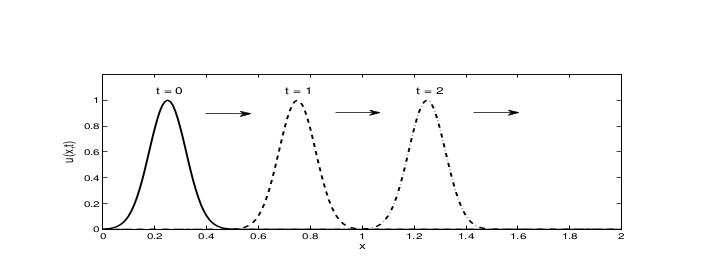
\includegraphics[width=15cm]{../Image/trueSolAdvection.png}
    \caption{Linear advection model: true solution $u(x, t)$}
    \label{trueSol}
    \end{center}
\end{figure}


\subsubsection{Perfect observations}
The value of the initial estimate $a_0$ is $a_0= 0.87116$. \\
As the name section indicates, the observations are perfects which means that no noise is adding in the observations. \\
The results is represented in the figure \ref{perfectObs} \cite{HybridSequential}.\\

\begin{figure}[h]
    \begin{center}
    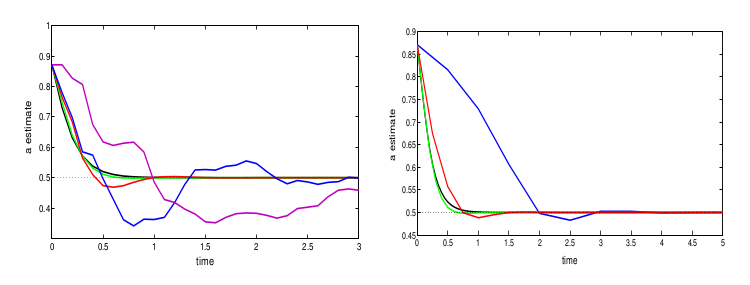
\includegraphics[width=9cm]{../Image/perfectObsAdvection.png}
    \caption{Perfect observations: parameter updates for initial estimate a = 0.87116.
(a) Varying the spatial frequency of observations: solid black line - observations at $2\Delta x$ intervals; solid green line -
observations at $5\Delta x$ intervals; solid red line - observations at $10\Delta x$ intervals; solid blue line - observations
at $25 \Delta x$ intervals; solid purple line - observations at $50\Delta x$ intervals. (b) Varying the temporal frequency
of observations: solid black line - observations every $5\Delta x$; solid green line - observations every $10\Delta x$; solid
red line - observations every$25\Delta t$; solid blue line - observations every $50\Delta t$.}
    \label{perfectObs}
    \end{center}
\end{figure}

\begin{itemize}
    

\item  Figure \ref{perfectObs} (a) shows the effect of varying the spatial frequency of observations for the initial estimate. Observations are assimilated every $10\Delta t$, with $\sigma_0^2 = 0.01$ and grid spacing between observations range from every $2\Delta x$ to every $25\Delta x$. The scheme performs extremely well.For observations taken every $2\Delta x$, $10\Delta x$ and $25\Delta x$ the scheme recovers the true value of a to a high level of accuracy. The quality of the state analysis is also high. To every 50 and 100 , the estimates take much longer to stabilise. With observations every $100\Delta x$ the $a$ estimate gets close to but never quite settles on the true value of $a$. 

\item  Figure \ref{perfectObs} (b), shows the effect of varying the temporal frequency of the observations for the same starting estimate $a_0$. Observations are taken every $5\Delta x$, and assimilated at intervals of $5\Delta t$, $10\Delta t$, $25\Delta t$ and $50\Delta t$. The results are similar to the previous experiment there is a differnce when the time when the time between successive assimilations is increased from every $5\Delta t$ to $10\Delta t$ to $25\Delta t$. For observations every $50\Delta t$ the a estimate takes slightly longer to converge. If this period is doubled again to $100\Delta t$ the scheme completely fails to recover $a$.
\end{itemize}

\subsubsection{Noisy observations}
In this section, we add noise in the observations. The noise is defined as Gaussian with mean zero and variance $\sigma_a^2$. And the results are represented in the figure \ref{noisyObs} \cite{HybridSequential}.
\begin{figure}[h]
    \begin{center}
    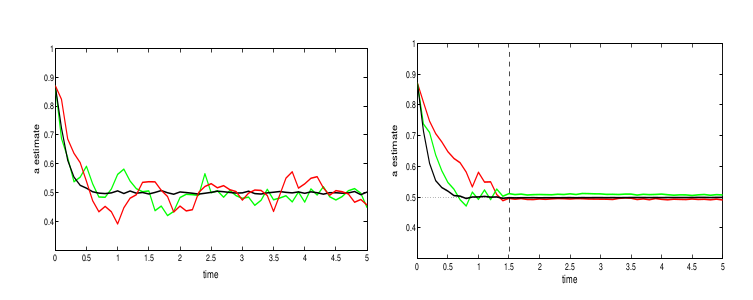
\includegraphics[width=9cm]{../Image/noisyObs.png}
    \caption{Imperfect observations: parameter updates for initial estimate $a = 0.87116$ (a) unaveraged estimates, and (b) time averaged estimates: solid black line $\sigma_0^2 = 0.001$; solid green line $\sigma_0^2 = 0.01$; solid red line $\sigma_0^2= 0.1$}
    \label{noisyObs}
    \end{center}
\end{figure}

\begin{itemize}
\item Figure \ref{noisyObs} (a) shows the parameter a estimates produced for error variance increasing from $\sigma_a^2=0.001$ to $\sigma_a^2=0.1$
The results is that when the observations are noisy, then resulting analysis and estimate parameters are also noisy. The amplitude of oscillations in $a$ increase as $\sigma_a^2$ is increased. When the $\sigma_a^2$, the state analysis is particularly messy. The oscillations are approximately centered around a true value $a$


\item In figure \ref{noisyObs} (b),the same experience above is repeated but with the $a$ estimates being averaged over a moving time
window of 20 timesteps.

\end{itemize}
%---------------------------------------------------------




%---------------------------------------------------------
\section{Conclusion}
A key difficulty in the construction of a data assimilation algorithm is specification of the background error covariances. These covariances play an important role in the filtering and spreading of observational
data and have a direct influence on the quality of the analysis

As the results obtained showed, the scheme performed well in all of the three
cases considered and was successful in recovering the parameter values we had specified to a good level of accuracy, even when the observational data were noisy. This had a positive impact on the skill of the forecast model and enabled more accurate predictions of the true model state.


%-------------------MIchi Part finished--------------------------------------

\newpage
\bibliographystyle{plain}
\bibliography{report}
\end{document}